\chapter{Project Implementation}
\section{Design Patterns}
\label{section:bloc-pattern}
The main architectural pattern used during the development of the mobile application is called BloC (Business Logic Component)~\cite{bloc-pattern}. It is a pattern created by Google, especially for Flutter framework. To manage the flow of data within an app, it uses Reactive Programming~\cite{reactive-programming}, which in simple terms, is programming with asynchronous data streams. Flutter user interfaces are composed of smaller parts called widgets. When a state of a widget changes, it is redrawn automatically on the screen. If there are lots of widgets used, their state can change multiple times, and they will be redrawn, sometimes unnecessary. That can lead to performance issues. This is where the BLOC comes into play. It helps to separate logic from the user interface while maintaining the Flutter reactive model of redrawing widgets.

A BLoC has two main components: Sinks and Streams, both of which are provided by a~StreamController. A Stream is a source of asynchronous data events, which provides a way to receive a sequence of events. These events can be user inputs, hover events, variables, click events, network requests, and others. A Sink is a place where data or events are added and can be read by a Stream. Everything in the application should be represented as a stream of events. Some widgets submit events to the BLoC, which acts as a middleman, and other widgets will receive and react to processed data, as shown in Figure~\ref{fig:bloc-pattern}.

\begin{figure}[htb]
    \centering
    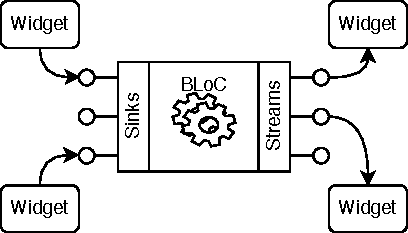
\includegraphics[width=0.5\textwidth]{fig04/bloc_pattern.pdf}
    \caption{Visual representation of the BLoC pattern (based on~\cite{bloc-image})} \label{fig:bloc-pattern}
\end{figure}

Using the BLoC pattern, we can manage the state of an application clearly, and it helps in writing concise and clean code. The user interface is separated from the business logic, which makes it easier to change the user interface without modifying the business logic.

\section{Project Management}
\paragraph{\large{GitKraken Glo}}\mbox{}\\[2pt]
All tasks created while developing the project were managed with GitKraken Glo Board~\cite{gitkraken-glo}. It is a Kanban board for task and issue tracking, which is fully integrated with GitKraken. It allows adding labels, descriptions, comments, assignees, and many others to created cards. As seen in Figure~\ref{fig:glo-board}, four statuses of tasks turned out to be enough for this system (backlog, on hold, doing, and done). Usage of the mentioned Kanban board simplified the development because it was easy to see what was already done and what still needs to be implemented.

\begin{figure}[htb]
    \centering
    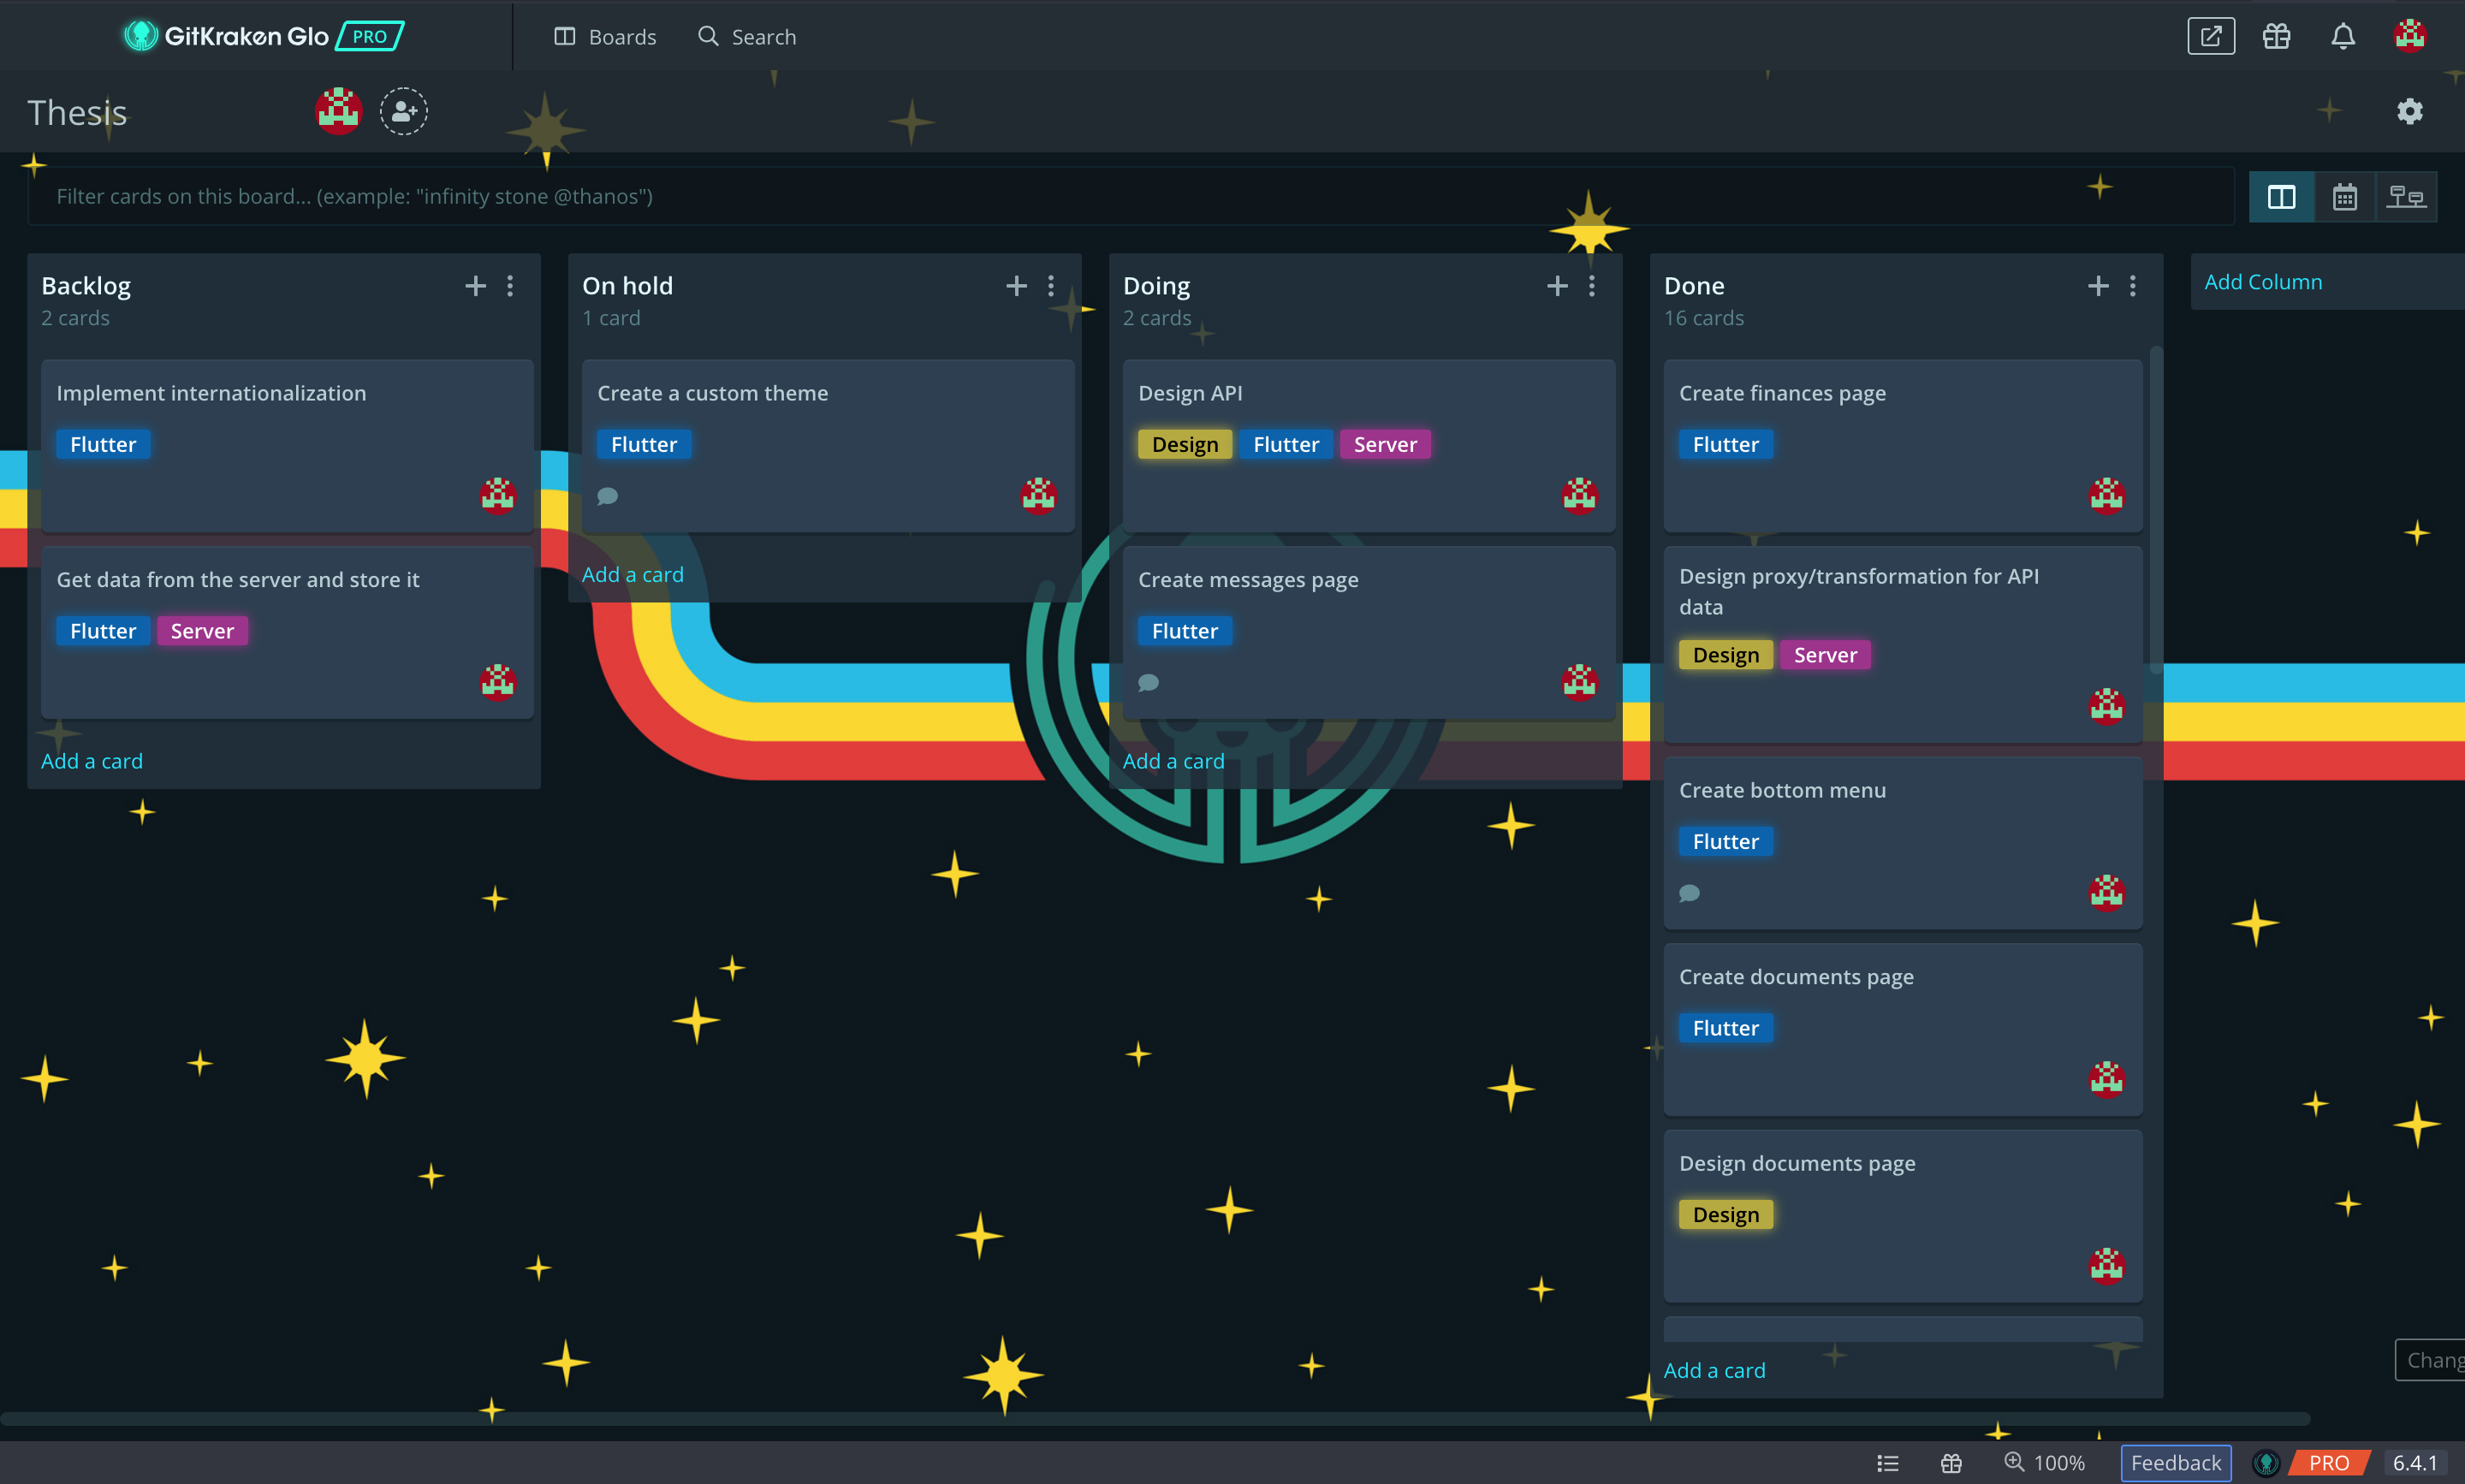
\includegraphics[width=.98\textwidth]{fig04/glo_board.png}
    \caption{An example of GitKraken Glo Board} \label{fig:glo-board}
\end{figure}

\paragraph{\large{GitFlow}}\mbox{}\\[2pt]
GitFlow was used to ease the development of tasks. It is a branching model for Git, created by Vincent Driessen~\cite{gitflow}. It makes parallel development very easy because it isolates new changes from finished work. The new development is done in feature branches. They are only merged back into the main code when the developer thinks that the code is ready for release. If a person is asked to switch from one task to another, all they need to do is commit changes and create a~new feature branch for the new task. When the task is done, they check out the original feature branch and can continue where they left off.
For the purpose of the project, the GitFlow was slightly altered. A new type of branch was introduced, a bugfix branch. All fixes were committed only to this type of branch. Figure~\ref{fig:gitflow} represents a part of the commit history for the mobile application, which uses GitFlow.

\begin{figure}[htb]
    \centering
    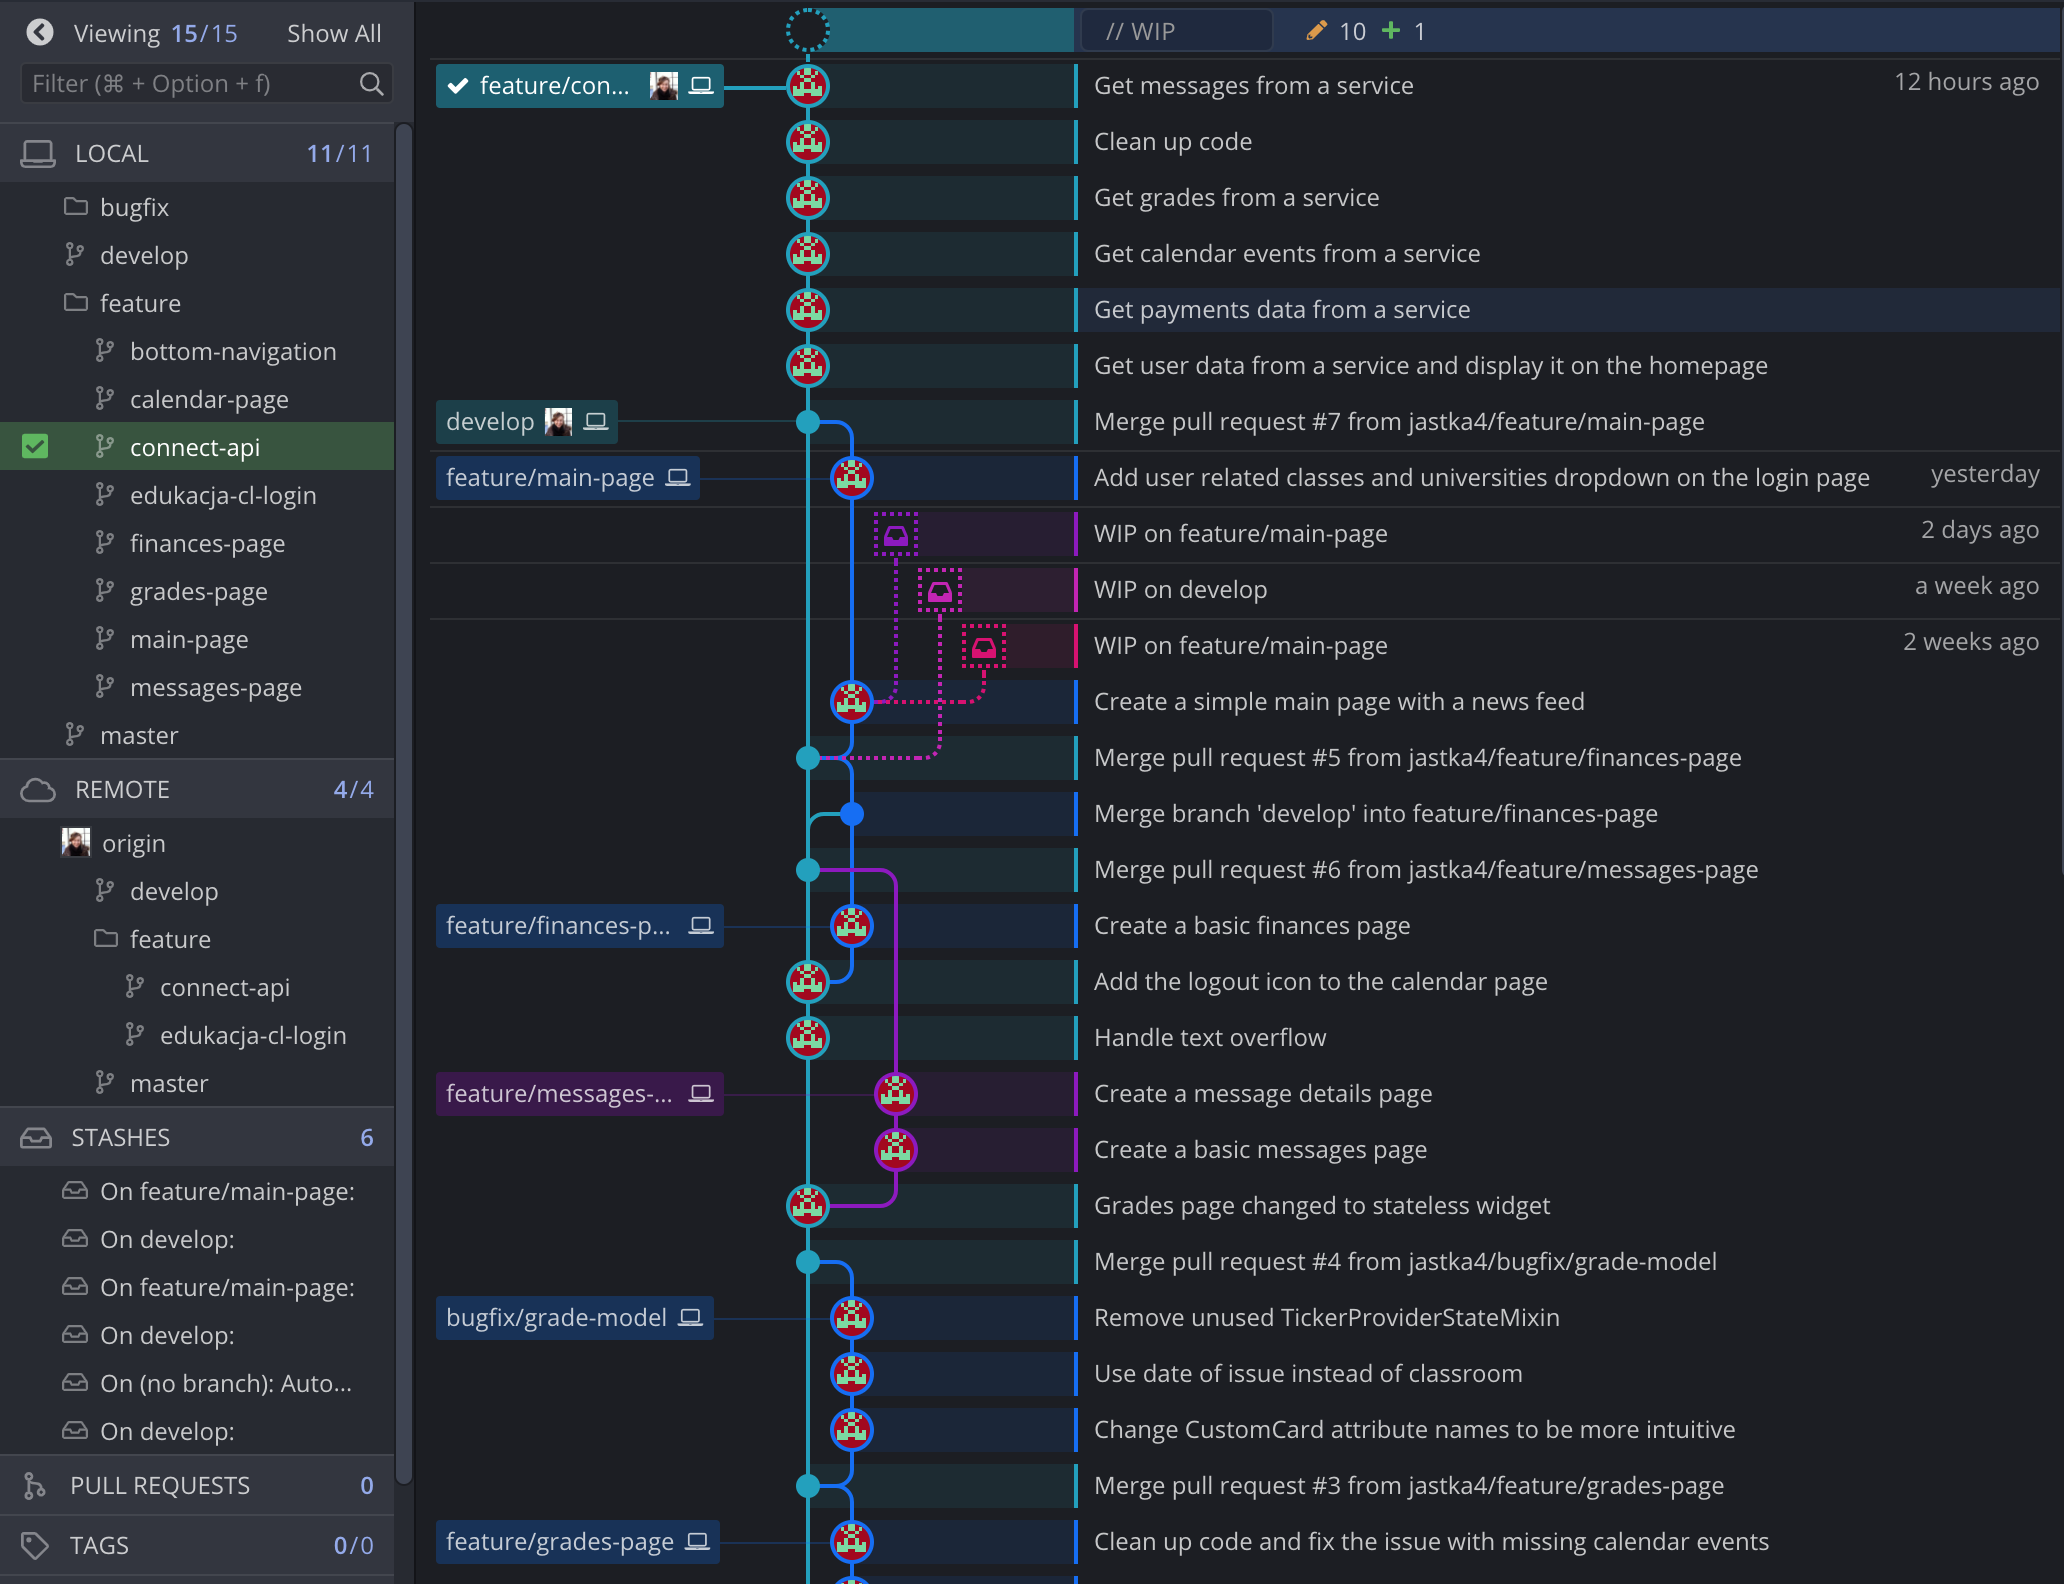
\includegraphics[width=.95\textwidth]{fig04/gitflow.png}
    \caption{Part of the commit history for the mobile application} \label{fig:gitflow}
\end{figure}

\section{Tools and Technologies}
\paragraph{\large{Flutter}}\mbox{}\\[2pt]
Flutter is an open-source toolkit created by Google~\cite{flutter}. It can be used to develop natively compiled applications for mobiles (iOS, Android), desktops (Mac, Linux, Windows, Google Fuchsia), and the web from a single codebase. Flutter's engine utilizes Google's Skia graphics library for low-level rendering. It is written primarily in C++. It also leverages platform-specific SDKs, for example, iOS and Android.

Flutter applications are created using the Dart language. The toolkit runs in the Dart virtual machine that features a just-in-time execution engine. It can be used while debugging an app to do a ``hot reload'', which modifies source files and then injects them into a~running application. Flutter added a stateful hot reload on top of it, wherein most cases, changes to source code can be reflected immediately in the working app without requiring a restart or any loss of state.

Release versions of Flutter apps are compiled with ahead-of-time (AOT) compilation on both iOS and Android, making Flutter's high performance on mobile devices possible~\cite{flutter-wiki}.

Creating UIs in Flutter involves using composition to assemble widgets from other widgets. According to the docs, ``A widget is an immutable description of part of a user interface''~\cite{flutter}. They define what their view should look like, given their current state and configuration. The widget rebuilds its description when it's state changes because the framework diffs against the previous representation to determine the minimal changes needed in the underlying render tree to transition from one state to the next.

Flutter aims to provide 120 frames per second (FPS) performance on devices capable of 120Hz updates and 60 FPS otherwise.

Complex widgets can be built from other smaller ones. An app is actually the largest widget of all of them, often called ``MyApp''. Text component is a widget, but so is its TextStyle, than defines things like color, size, font-weight, and family. Some widgets represent things, others, like TextStyle, represent characteristics. There are also ones that do something, like StreamBuilder and FutureBuilder.

An alternative option to using widgets is to use the Foundation library's methods directly. They can be used to draw text, shapes, and imagery directly on the canvas. One of the frameworks that utilized this is the open-source Flame game engine.

\paragraph{\large{Dart}}\mbox{}\\[2pt]
Dart is a client-optimized programming language developed by Google~\cite{dart}. It is multiplatform and can be used to build desktop, mobile, backend, and web applications.

It is object-oriented, class defined, garbage-collected language. It uses a C-style syntax and can be transcompiled into JavaScript. It supports abstract classes, interfaces, mixins, static typing, reified generics, and a sound type system.

Dart code can be compiled ahead-of-time into machine code. Applications build with Flutter, a mobile app SDK built with Dart, are deployed to app stores as AOT compiled Dart code.

Dart version 2.6 was accompanied by a new extension dart2native. It allows composing a Dart program into self-contained executables on the macOS, Linux, and Windows desktop platforms. Earlier, this feature only exposed capability on iOS and Android mobile devices via Flutter~\cite{dart-wiki}.

\paragraph{\large{SQLite}}\mbox{}\\[2pt]
SQLite is a relational database management system contained in a C-language library~\cite{sqlite}. It is embedded into the end program, unlike many other database management systems. It is built into most computers, all mobile phones and is bundled inside lots of applications that people use every day. It is a popular selection as an embedded database software for client/local storage in application software such as web browsers. It is one of the most used database engines, as it is used today by several widespread browsers, embedded systems, such as mobile phones, operating systems, among others. SQLite has bindings to many programming languages.

SQLite is ACID-compliant and follows PostgreSQL syntax while implementing most of the SQL standard. It uses weakly and dynamically typed SQL syntax that does not guarantee the domain integrity. A string can be inserted into a column defined as an integer. SQLite will try to convert data between formats when appropriate, for example, the string ``1234'' into an integer. However, it does not guarantee such conversion and will store the data as-is if such conversion is not possible~\cite{sqlite-wiki}.

\paragraph{\large{Android Studio}}\mbox{}\\[2pt]
Android Studio is an integrated development environment created by Google and built on JetBrains' IntelliJ IDEA software~\cite{android-studio}. It was specially designed for Android development. It can be downloaded on macOS, Windows, and Linux based operating systems. Previous versions of Android Studio were based on Eclipse IDE.

Flutter apps can be built using any text editor combined with Flutter command-line tools. It is best to use the Flutter plugin with Android Studio. The plugin provides users with, for example, syntax highlighting, code completion, widget editing assist, run and debug support.

\paragraph{\large{Java}}\mbox{}\\[2pt]
Java is a general-purpose, object-oriented, class-based programming language~\cite{java}. It lets developers write once, run anywhere, so it can run on all platforms that support it without the need for recompilation.  It has been designed to have as few implementation dependencies as possible. Java applications are usually compiled into bytecode that can be run on any JVM, regardless of the architecture of the computer. The syntax of Java is similar to C++ and C, but it has fewer low-level facilities than either of them. According to GitHub, Java is currently one of the most popular programming languages used, particularly for client-server web applications~\cite{java-wiki}.

\paragraph{\large{Spring Framework}}\mbox{}\\[2pt]
Spring Framework is an open-source Java platform and a container for inversion of control~\cite{spring}. Its core features can be used in developing any Java applications. There are also extensions for creating web applications on top of the Java Enterprise Edition (Java EE) platform. The framework targets to make Java EE development more comfortable to use and promotes good programming practices by enabling a POJO-based programming model. Even though the framework does not impose any specific programming model, it has become popular in the Java community as an add-on or even a replacement for the Enterprise JavaBeans model.

Spring Boot is an open-source micro-framework maintained by Pivotal company~\cite{spring-boot}. It is pre-configured by the Spring team with the best configuration possible and use of the Spring platform and third-party libraries so that developers can quickly get started without wasting time on preparation.

Spring Cloud Config provides client and server-side support for externalized configuration in distributed systems~\cite{spring-cloud-config}. The Config Server is a central spot to manage external properties for apps across all environments. The configuration can be used with any application running in any language.

The Spring Web MVC platform provides MVC (Model-View-Controller) architecture and components that can be used to create loosely connected and flexible web applications~\cite{spring-mvc}. The MVC pattern separates various aspects of the application (business logic, user interface logic, and input logic), providing a loose relationship between these.

\begin{itemize}
    \item Model - a POJO that encapsulates the application data;
    \item View - responsible for rendering the model data;
    \item Controller - responsible for processing user requests, building the appropriate model, and passing it to the view for rendering.
\end{itemize}

\paragraph{\large{Jolt}}\mbox{}\\[2pt]
Jolt (JsOn Language for Transform) is a transformation library written in Java~\cite{jolt}. It allows developers to convert one JSON structure to another using a schema created in JSON. The tool provides a set of transformation types:

\begin{itemize}
    \item shift - copies data from input to the output tree;
    \item default - applies default values to the tree;
    \item remove - removes data from the tree;
    \item sort - sorts map keys alphabetically;
    \item cardinality - adjusts the cardinality of input data.
\end{itemize}

Each of the types has its DSL, which is called a specification, that defines the new structure for outgoing JSON data.

A basic approach for converting JSON to JSON in Java is to use XSLT or STX. The conversion sequence would look like this:
\begin{center}
\textbf{JSON -> XML -> XSLT/STX -> XML -> JSON}
\end{center}

With Jolt, the conversion sequence is simplified and looks like this:
\begin{center}
\textbf{JSON -> Specification JSON -> JSON}
\end{center}

The out-of-the-box Jolt should be able to do most of the structural transformation. Any complex transformation logic which cannot be expressed in standard terms can be plugged in via Java extension class with Jolt.

\paragraph{\large{JSON}}\mbox{}\\[2pt]
JSON (JavaScript Object Notation) is a lightweight data-interchange text format that is easy for a~machine to parse and generate, but also for humans to read and write~\cite{json}. It is entirely language-independent and uses array data types and attribute-value pairs to transmit data objects. It is a~widespread data format and serves as a replacement for XML in AJAX systems.

\paragraph{\large{YAML}}\mbox{}\\[2pt]
AML Ain't Markup Language (YAML) is a data serialization language that has a human-readable format~\cite{yaml}. It is commonly used for configuration files and in applications where data is being transmitted or stored. It targets many of the same communication applications as XML but has minimal syntax. It uses both Python-style indentations to indicate nesting, and a~more compact format that uses ``[]'' for lists and ``\{\}'' for maps making YAML 1.2 a superset of JSON.

\paragraph{\large{MockServer}}\mbox{}\\[2pt]
MockServer is an open-source platform used to mock systems via HTTP or HTTPS~\cite{mockserver}. It was designed to simplify integration testing by mocking systems such as web services or websites. It also helps in developing code against a service that is not complete or is unstable.

\paragraph{\large{Docker}}\mbox{}\\[2pt]
Docker is a platform for developing, shipping, and running applications~\cite{docker}. It enables to separate applications from the infrastructure so that they can be delivered quickly. It also provides an ability to package and run applications in a loosely isolated environment called a container. Many different containers can be run simultaneously on a given host.

Docker team also made Docker Compose. It is a tool for defining and launching Docker applications using multiple containers~\cite{docker-compose}. It utilizes YAML files to configure the application’s services. Then they can be created and started with just a single command.

\section{Database Configuration}
The database is elementary and does not contain any relations. That is why the model-first approach was used during the implementation. All tables are created on a smartphone during the first run of the mobile application. The \texttt{DBProvider} class presented in Listing~\ref{list:db-provider} is a singleton and creates a new database only if none exists on the device. If the \texttt{universityTable.db} exists, it is opened and used throughout the application.

\lstinputlisting[label=list:db-provider,caption=The database provider class]{code04/db_provider.dart}

 The \texttt{initDB} method creates new tables with the previously created scripts. An example of a~script creating a user table is shown in Listing~\ref{list:create-user-table}.

\lstinputlisting[label=list:create-user-table,caption=SQL script to create a user table]{code04/create_user_table.dart}

\section{Mobile Application Implementation}
The mobile application is the largest part of the project. It uses Flutter framework and the BLoC pattern, which imposes a particular folder structure (Fig.~\ref{fig:flutter-folder-structure}):
\begin{itemize}
    \item \texttt{.dart\_tools} -- used by pub and other tools.
    \item \texttt{.idea} -- contains IntelliJ’s project specific settings files.
    \item \texttt{android} -- stores Android native project that is used when building the app for Android devices.
    \item \texttt{build} -- holds the compiled code of the Flutter application.
    \item \texttt{images} -- contains all image assets used by the app. It could also be placed inside the \texttt{lib} folder.
    \item \texttt{ios} -- only available when working on macOS. Stores XCode iOS native project that is used when building the app for iOS devices.
    \item \texttt{lib} -- holds Dart files containing Flutter application code.
    \item \texttt{blocs} -- composed of different BLoC components used throughout the app. Each of them has a dedicated folder for storing the main BLoC logic, event, and state classes.
    \item \texttt{common} -- contains common files (providers, helpers, enums).
    \item \texttt{dao} -- a place with all DAOs.
    \item \texttt{models} -- keeps all models.
    \item \texttt{repositories} -- a folder containing repositories that are used by components to fetch data from the API or database, depending on the availability. Inside each of the files is a logic determining if users have an active connection to the Internet. They also store downloaded data in a database.
    \item \texttt{services} -- holds services responsible for fetching data from the API.
    \item \texttt{ui} -- stores all UI elements that are divided into reusable \texttt{components} and \texttt{screens} holding views.
    \item \texttt{tests} -- contains all tests written for the application.
\end{itemize}
\begin{figure}[t]
    \centering
    \includegraphics[width=.85\linewidth]{fig04/flutter-folder-structure.png}
    \caption{Folder structure of the Flutter application}
    \label{fig:flutter-folder-structure}
\end{figure}

In addition to these structures, there is a \texttt{.gitignore} file used for the program versioning. \texttt{pubspec.yaml} is a place where developers can provide all the required dependencies and project configuration.

% ---------------------------------------------

\paragraph{\large{BLoC}}\mbox{}\\[2pt]
The first type of elements are the Business Logic Components (see Section~\ref{section:bloc-pattern}). They manage the flow of data within the application using asynchronous data streams. In the context of the program, a BLoC takes a stream of events as an input and transforms them into a stream of states as output (Fig.~\ref{fig:bloc-diagram}).

\begin{figure}[htb]
    \centering
    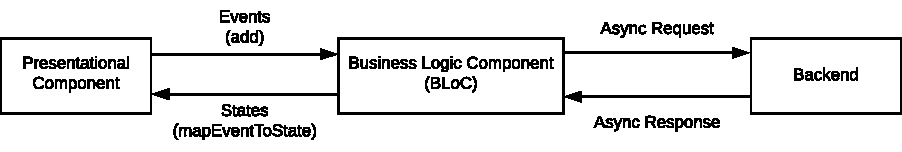
\includegraphics[]{fig04/bloc_diagram.pdf}
    \caption{High-level BLoC diagram (based on~\cite{bloc-diagram})}
    \label{fig:bloc-diagram}
\end{figure}

Events are the input of a BLoC. They are often UI events, such as pressing a button. Events are added and then converted to states. The Listing~\ref{list:login-event} shows an example of the event implementation. It is a simple object that stores \texttt{username}, \texttt{password}, and \texttt{university}. It has a~simple constructor and a \texttt{toString} method. \texttt{Equatable} overrides \texttt{==} and \texttt{hashCode} so objects can be easily compared.

\lstinputlisting[label=list:login-event,caption=Login event]{code04/login_event.dart}

States are the output of a BLoC. All presentation components can listen to the state stream and redraw their parts based on the given state. Listing~\ref{list:login-state} represents a simple class used for login, with multiple states available. Each of them can have different attributes and implementation; for example, \texttt{LoginFailure} differs from the rest.

\lstinputlisting[label=list:login-state,caption=Login state]{code04/login_state.dart}

The last but not least is the actual logic of the BLoC (List.~\ref{list:login-bloc}). It uses previously defined state and event classes, and it has two attributes (\texttt{userRepository} and \texttt{authenticationBloc}). The initial state of the BLoC is set to \texttt{LoginInitial}. Besides the constructor and a simple getter, there is a \texttt{mapEventToState} method. It converts the incoming events into states which are consumed by the presentation layer. If the event is \texttt{LoginButtonPressed}, the state is changed into \texttt{LoginLoading}. Next, it tries to authenticate the user and adds a \texttt{LoggedIn} event for the \texttt{authenticationBloc}. The last part is to change the state into the initial state. If any error occurs, the state is changed to \texttt{LoginFailure}, and the details of the error are passed there.

\lstinputlisting[label=list:login-bloc,caption=Login BLoC]{code04/login_bloc.dart}

% ---------------------------------------------

\paragraph{\large{DAO}}\mbox{}\\[2pt]
Another type of components used in the system are DAOs. It is a pattern that provides an abstract interface for communication between the application and the database. DAO methods are very similar, and an example is shown in Listing~\ref{list:grades-dao}. The first step is to establish a connection to SQLite. After it has been successful, we query the database, map the results to \texttt{Grade} object, and return the list.

\lstinputlisting[label=list:grades-dao,caption=Getter method defined in the grades DAO]{code04/grades_dao.dart}

% ---------------------------------------------

\paragraph{\large{Model}}\mbox{}\\[2pt]
The model is a simple data structure with lots of properties. It has a constructor, \texttt{toMap}, and \texttt{toString} methods. Besides them, there are factory constructors capable of creating objects from JSON (List.~\ref{list:payment-model}) or map structure.

\lstinputlisting[label=list:payment-model,caption=Payment factory constructor]{code04/payment_model.dart}

% ---------------------------------------------

\paragraph{\large{Repository}}\mbox{}\\[2pt]
The next type is the repository, which is responsible for fetching data from the database or API, depending on the availability. The \texttt{getCalendarEvents} method (List.~\ref{list:calendar-repository}) obtains customer's data such as username and university, which are required by the API. Next, we verify if the mobile device has an active Internet connection. If not, we get calendar events from the local database. If the user has access to the web, we try to fetch events from the service and update the local database.

\lstinputlisting[label=list:calendar-repository,caption=Getter method defined in the calendar repository]{code04/calendar_repository.dart}

% ---------------------------------------------

\paragraph{\large{Service}}\mbox{}\\[2pt]
The service is a component responsible for fetching data from an external API. \texttt{fetchCalendarEvents} method (List.~\ref{list:calendar-service}) retrieves calendar events for selected dates and a~student. It sends a POST request with JSON body and waits for a response. After it successfully obtained the data, it maps the response to the \texttt{CalendarEvent} and returns it. If the \texttt{statusCode} is different from 200, it throws an exception.

\lstinputlisting[label=list:calendar-service,caption=Calendar service]{code04/calendar_service.dart}

% ---------------------------------------------

\paragraph{\large{UI}}\mbox{}\\[2pt]
The last type of components in the application are UI widgets. They allow building views by simply stacking widgets on top of each other. Listing~\ref{list:home-screen} shows a \texttt{build} method of the home screen. It draws a \texttt{Scaffold} with an app bar build by a private method \texttt{\_buildAppBar}. Under it, there is a \texttt{Container} with a scrollable view, that has two rows. The first one is the profile info, and the second is the news feed. It also uses \texttt{\_authenticationBloc} to manage user data.

\lstinputlisting[label=list:home-screen,caption=Build method of the home screen]{code04/home_screen.dart}

\section{Server Implementation}
The server is composed of two server modules (Fig.~\ref{fig:server-folder-structure}): configuration (\texttt{*-server-config}) and transformation (\texttt{*-server-client}). Both were created with Spring Framework (Spring MVC, Spring Boot, and Spring Cloud Config). The main project has its own \texttt{pom.xml} with a simple parent config. There are two separate folders for each of the modules. There is a~global \texttt{.gitignore} file for versioning of the program. \texttt{.idea} and \texttt{.mvn} contain project-specific settings for IntelliJ IDEA and Maven.

\begin{figure}[htb]
    \centering
    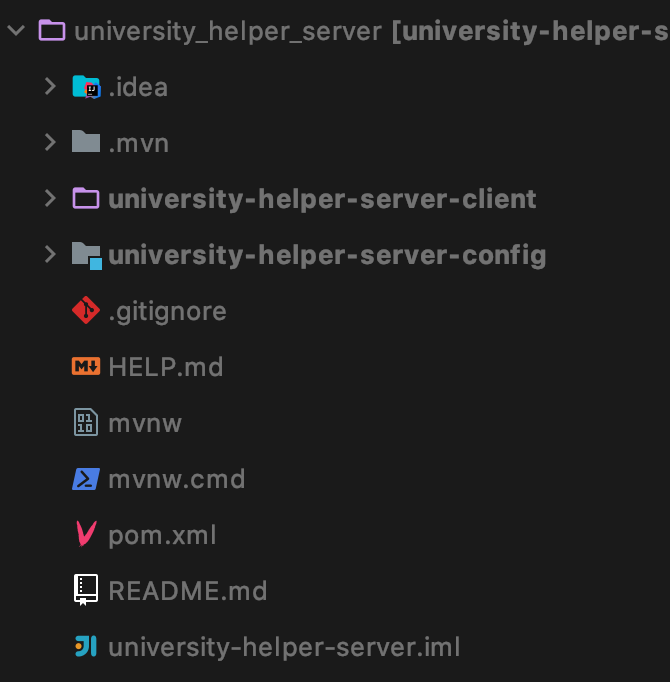
\includegraphics[width=.44\linewidth]{fig04/server-folder-structure.png}
    \caption{Folder structure of the transformation server}
    \label{fig:server-folder-structure}
\end{figure}

Figure~\ref{fig:server-config-folder-structure} represents a folder structure for the first of the modules. It includes:
\begin{itemize}
    \item \texttt{java} -- contains a package with the main class that acts as an entry point for the entire program.
    \item \texttt{resources} -- keeps a properties file, which is a configuration for the Spring Cloud Config.
    \item \texttt{test} -- contains all tests written for the module.
\end{itemize}

\begin{figure}[htb]
    \centering
    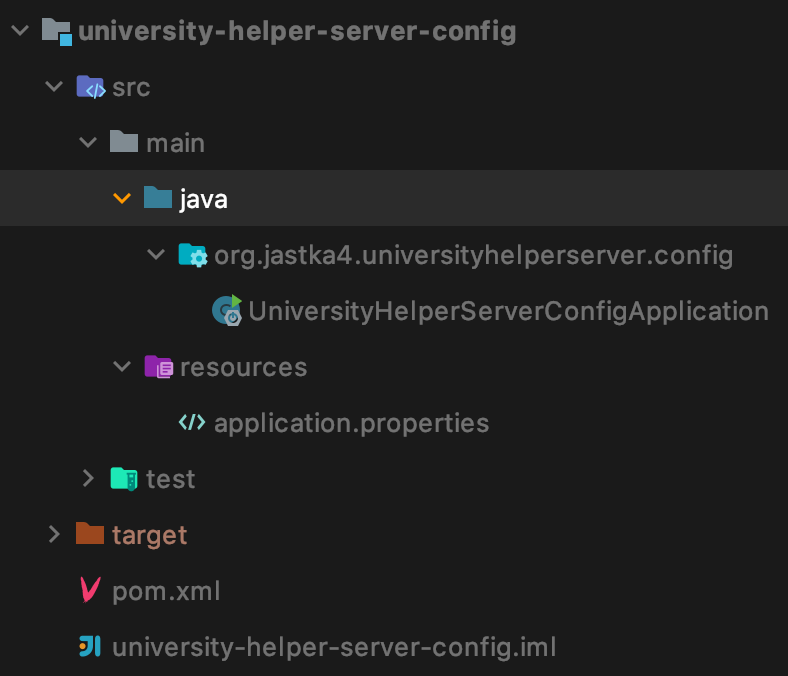
\includegraphics[width=.46\linewidth]{fig04/server-config-folder-structure.png}
    \caption{Folder structure of the configuration module}
    \label{fig:server-config-folder-structure}
\end{figure}

The \texttt{UniversityHelperServerConfigApplication} file (see Listing~\ref{list:server-config-main-class}) is the main class of the configuration module. \texttt{@EnableConfigServer} annotation was used to enable Spring Cloud Config for the program. It allows to share the specified configuration between many microservices and applications.

\begin{lstlisting}[label=list:server-config-main-class,caption=Server configuration main class, basicstyle=\footnotesize\ttfamily]
@SpringBootApplication
@EnableConfigServer
public class UniversityHelperServerConfigApplication {

	public static void main(String[] args) {
		SpringApplication.run(UniversityHelperServerConfigApplication.class, args);
	}
}
\end{lstlisting}

The properties for the Spring Cloud Config (see Listing~\ref{list:spring-cloud-config-properties}) have the following meanings:
\begin{itemize}
    \item \texttt{server.port} -- sets the server on which the module will run.
    \item \texttt{spring.cloud.config.server.git.uri} -- specifies the URI of the remote repository containing the property files that will be served by the configuration service.
    \item \texttt{spring.cloud.config.server.git.clone-on-start} -- determines whether the configuration from the repository should be cloned when starting the module.
\end{itemize}

\begin{lstlisting}[label=list:spring-cloud-config-properties,caption=Spring Cloud Config properties, basicstyle=\footnotesize\ttfamily]
server.port=8888
spring.cloud.config.server.git.uri=https://github.com/jastka4/university-helper-config
spring.cloud.config.server.git.clone-on-start=true
\end{lstlisting}

Figure~\ref{fig:server-client-folder-structure} represents a folder structure for the second of the modules. It includes:
\begin{itemize}
    \item \texttt{common} -- a folder containing enums available in the system, a transformation POJO used to store configuration from the YAML file, and university constants required for transformation. There is also a new exception type created specifically for this system.
    \item\texttt{config} -- contains transformation configuration class. It is a simple POJO that stores a list of every type, for example, payments, finances, et cetera.
    \item \texttt{controllers} -- a place where all controllers are placed. In this case there is only the main one, which handles every incoming request.
    \item \texttt{services} -- holds services for handling requests and transformations. It contains only interfaces, and the \texttt{impl} folder, which stores implementations of the said interfaces.
    \item \texttt{resources} -- keeps a properties file, which is a configuration read by Spring Cloud Config.
    \item \texttt{test} -- contains all tests written for the module.
\end{itemize}
\begin{figure}[b]
    \centering
    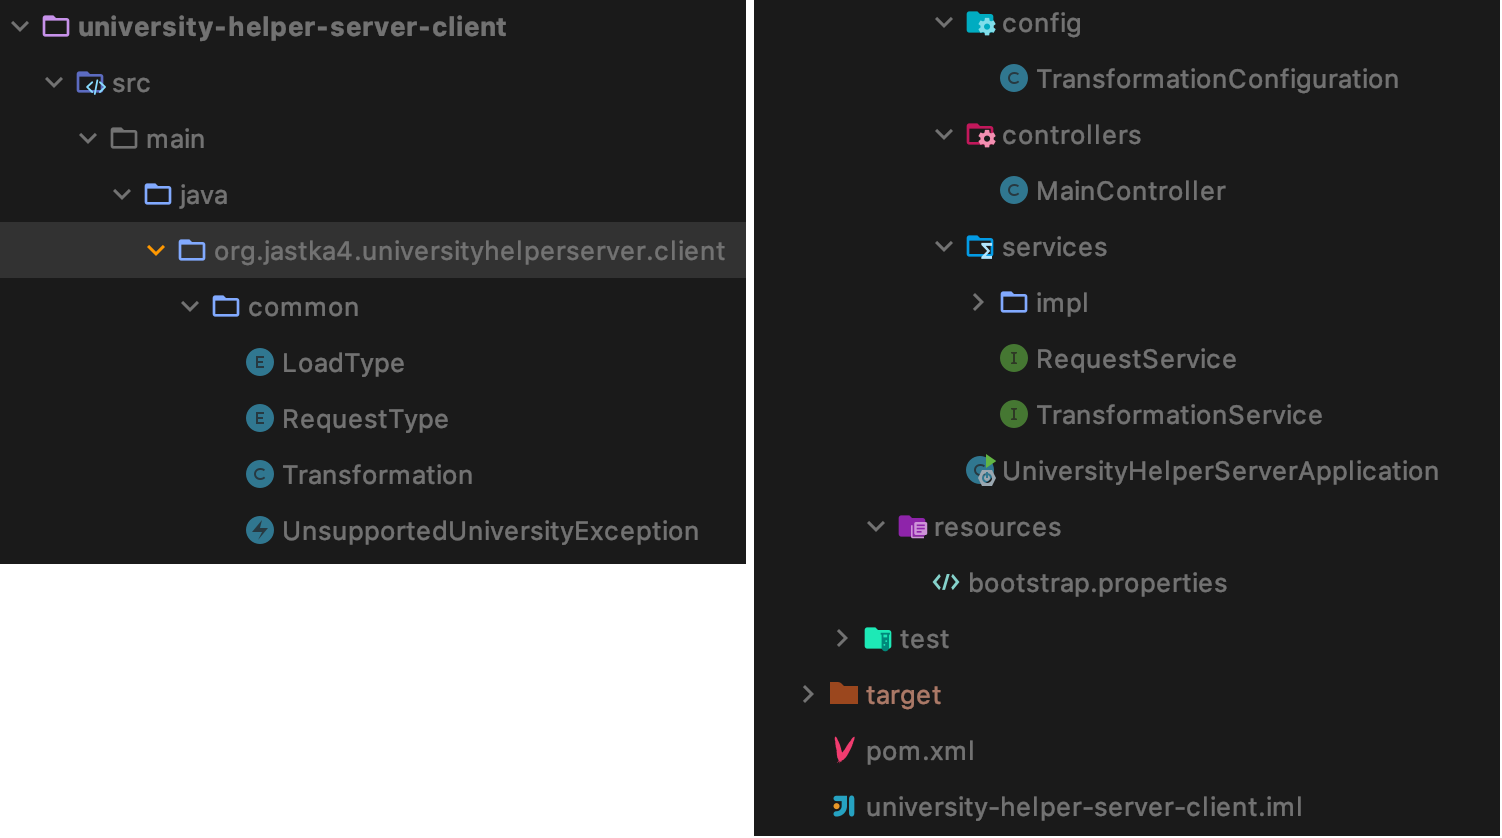
\includegraphics[width=.75\linewidth]{fig04/server-client-folder-structure.png}
    \caption{Folder structure of the transformation module}
    \label{fig:server-client-folder-structure}
\end{figure}

In addition to these structures, there is a \texttt{UniversityHelperServerApplication} file that acts as an entry point for the entire program. The last but not least is \texttt{pom.xml}, which contains information, configuration, build directory, source directory, test source directory, plugins, dependencies, et cetera used by Maven to build the module.

Method shown in Listing~\ref{list:calendar-controller} is responsible for handling all calendar requests. It reads the incoming JSON and sends it to \texttt{sendRequestToUniversityApi} method with a parameter that indicates that the request was of calendar type. If exception happens during the execution 400 status is returned with a JSON response containing the error message.

\lstinputlisting[label=list:calendar-controller,caption=Method that handles all calendar requests]{code04/calendar_controller.dart}

The \texttt{sendRequestToUniversityApi} method shown in Listing~\ref{list:send-request} is responsible for sending a request to the chosen university's API and returning the response. The first step is to transform the input JSON to the format expected by the API. To do it, we need to get the university from the request and store it for future use. The next action is to send the transformed request and get the response. The last step is to transform the answer to the format readable by the mobile application. If the initial request contains a university not supported by the configuration or the config is missing, the \texttt{UnsupportedUniversityException} is thrown.

\lstinputlisting[label=list:send-request,caption=Method that handles requests for university APIs]{code04/send_request.dart}

The primary method used for transformation is shown in Listing~\ref{list:transform-json}, and it utilizes the functions of the Jolt library. First, the request must be converted from a string to map of strings required by the library. Then we check if JSON is a request or response from the API and we get the matching transformation. Two last steps are to create the \texttt{Chainr} object from the transformation obtained in the previous step and to finally transform the JSON input and return it as a~string.

\lstinputlisting[label=list:transform-json,caption=Method transforming JSON]{code04/transform_json.dart}
